\begin{center}
    \addcontentsline{toc}{section}{ГЛАВА 3. SLAM НА ПРАКТЫЦЫ}
    \section*{ГЛАВА 3. \\ SLAM НА ПРАКТЫЦЫ}
\end{center}

Рэалізацыі алгарытмаў, разгледжаных у папярэдняй главе, даступныя ў вольным доступе
як праекты з адкрытым зыходным кодам. Аўтары каментуюць публікацыю як адначасова
унёсак у SLAM супольнасць і сродак для даследчыкаў з памежных галінаў \cite{murORB2}.

У супольнасці робататэхнікаў папулярнасцю карыстаецца ROS - аперацыйная сістэма для
распрацоўкі прыкладанняў для робатаў.

\vspace{5mm}

\addcontentsline{toc}{subsection}{3.1 ROS}
\subsection*{3.1 ROS}

ROS (The Robot Operating System) - фрэймворк для напісання праграмнага забеспячэння
для робатаў, з'яўляецца наборам інструментаў, бібліятэкаў і
канвенцыяў для зручнай і надзейнай працы з робатамі (\cite{288}). Патрэбнасць у фрэймворку ўзнікла
праз той факт, што стварэнне праграмнага забеспячэння для робатаў -
вельмі складаны і шматэтапны працэс; уніфікацыя спосабу камунікацый паміж часткамі вялікай
сістэмы дазваляе камандам працаваць над навігацыяй, рухам і зрокам робата асобна.

ROS пабудаваны на ідэі кліент-сервернага ўзаемадзеяння, што спрашчае працу ў размеркаваных
сістэмах, хаця і можа часам падавацца залішнім пры запуску на адной лакальнай машыне.

У аснове ROS ляжаць:

\begin{itemize}
  \item нізкаўзроўневы інтэрфейс перадачы паведамленняў,
  \item ананімная і асінхронная сістэма публікацыі і падпіскі на паведамленні,
  \item магчымасць рэалізацыі RPC для сінхроннага выкліку метадаў іншых пакетаў,
  \item глабальнае сховішча ключэй і значэнняў,
  \item зручныя сродкі дыягностыкі,
  \item інструменты для працы з ROS-ам праз графічны інтэрфейс: \textit{rviz}, \textit{rqt}.
\end{itemize}

Усе гэтыя ўласцівасці ROS-а робяць распрацоўку зручнай і лёгка ўбудоўваемай ў іншыя сістэмы.
Вялікая колькасць SLAM-алгарытмаў рэалізаваныя менавіта пад ROS і могуць не мець
уласных сродкаў візуалізацыі альбо ўводу дадзеных.

\addcontentsline{toc}{subsection}{3.2 Даследванне збежнасці ORB-SLAM}
\subsection*{3.2 Даследванне збежнасці ORB-SLAM}

У працэсе знаёмства з разнастайнымі SLAM-рэалізацыямі я правёў даследванне збежнасці
пазіцый камер у прасторы на прыкладзе ORB-SLAM. Сутнасць эксперыментаў заключалася ў наступным:
\begin{itemize}
  \item Запусціць алгарытм (у нашым выпадку - ORB-SLAM) на наборы дадзеных. У прыведзеных ніжэй выніках
  я выкарыстоўваў датасэт \textit{freiburg1\_desk} апублікаваны ў \cite{sturm12iros}.
  \item Пасля кожнага наступнага дададзенага здымка праверыць, ці была дададзеная новая камера.
  У выпадку, калі была - выгрузіць вонкавыя параметры ўсіх камераў, захаваць.
  \item Пасля таго, як усе дадзеныя прайшлі праз алгарытм, мы атрымалі мноства
  пазіцыяў камер, зарэгістраваных у розныя моманты часу. Пачынаем працу з гэтым дадзенымі.
  \item Для кожнай камеры знаходзім мноства яе пазіцый і сартыруем іх па часе. Пазіцыю, атрыманую
  ў канцы выканання алгарытма, прымаем за эталонную.
  \item Для кожнай камеры вылічваем яе ``блізкасць'' да эталоннай пазіцыі асобна па пазіцыі
  ў прасторы і па павароце. Адлегласць паміж пазіцыямі ў прасторы вылічваецца пры дапамозе
  Эўклідавай адлегласці \eqref{eq:euclidean-distance}, адлегласць паміж паваротамі, кожны з якіх
  задаецца кватэрніонам, вылічваецца па формуле \eqref{eq:quaternions-distance}. Адлегласць паміж
  паваротамі - значэнне памеру вугла, паварот на які прывядзе адзін кватэрніон у іншы.

  \begin{equation} \label{eq:euclidean-distance}
    d(a,b) = \sqrt{(a_x-b_x)^2 + (a_y-b_y)^2 + (a_z-b_z)^2}
  \end{equation}

  \begin{equation} \label{eq:quaternions-distance}
    d(q_1,q_2) = \arccos(2(q_1,q_2)^2-1)
  \end{equation}

  дзе $ a_{q_i}^2+b_{q_i}^2+c_{q_i}^2+d_{q_i}^2 = 1 $

  \item Далей праводзіцца аналіз дадзеных, атрыманых на папярэдніх кроках.
  Графічна дадзеныя прадстаўленыя на малюнках \ref{fig:conv-t-total} - \ref{fig:conv-q-histogram}.
  На кожным з графікаў \ref{fig:conv-t-total} - \ref{fig:conv-q-histogram} па восі абсцысаў
  адкладзены час: $0.0$ - момант, калі камера ўпершыню была размешчаная, $1.0$ - момант, калі
  камера была размешчаная на сцэне канчаткова і больш не ўдасканальвалася. Кожны графік (адзін колер) на
  малюнках \ref{fig:conv-t-total}, \ref{fig:conv-q-total} адпавядае адной камеры.
  Малюнкі \ref{fig:conv-t-histogram}, \ref{fig:conv-q-histogram} - гістаграмы, пабудаваныя па дадзеных
  для пазіцыяй і паваротаў камераў у прасторы адпаведна і з'яўляюцца абагульненнем малюнкаў \ref{fig:conv-t-total}
  і \ref{fig:conv-q-total}. Натуральна, што ўсе графікі сустракаюцца ў нулі ў момант часу $1.0$,
  бо ў гэты момант былі сфармаваныя эталонныя пазіцыі і павароты.

  \item Негледзячы на тое, што некаторыя камеры паводзяць сябе дастаткова дзіўным чынам і напрацягу доўгага
  часу пераходзяць паміж двумя станамі, агульная тэндэнцыя да збежнасці пазіцыяў і паваротаў камер
  да сваіх фінальных становішчаў добра праглядаецца.

\end{itemize}

Правядзенне эксперымента запатрабала рэалізацыю дадатковых метадаў у ORB-SLAM, а таксама
распрацоўку дапаможных утылітаў пад ROS.

\begin{figure}[H]
\centering
\begin{minipage}{.5\textwidth}
  \centering
  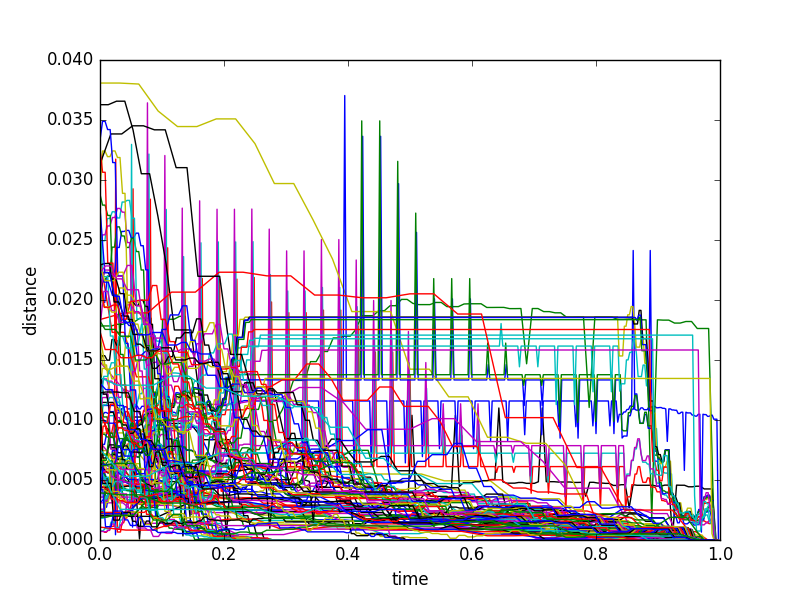
\includegraphics[width=\linewidth]{a__t_total}
  \captionsetup{labelformat=empty}
  \captionof{figure}{Мал. \arabic{figure}: збежнасць пазіцый камер}
  \label{fig:conv-t-total}
\end{minipage}%
\begin{minipage}{.5\textwidth}
  \centering
  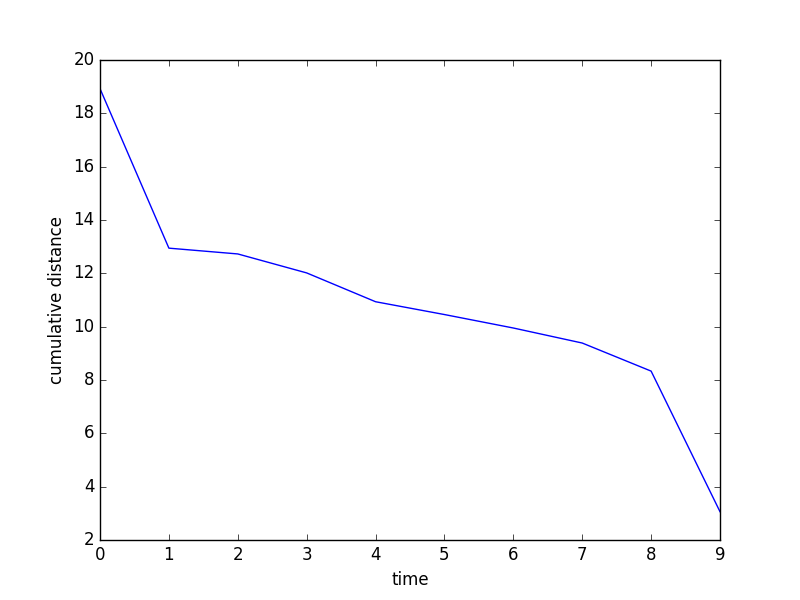
\includegraphics[width=\linewidth]{a__t_histogram}
  \captionsetup{labelformat=empty}
  \captionof{figure}{Мал. \arabic{figure}: адпаведная гістаграмма}
  \label{fig:conv-t-histogram}
\end{minipage}
\end{figure}

\begin{figure}[H]
\centering
\begin{minipage}{.5\textwidth}
  \centering
  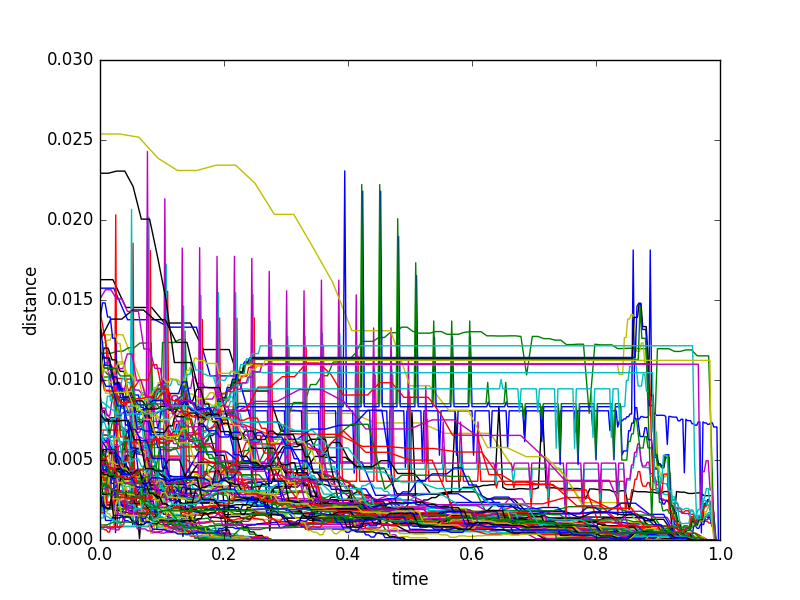
\includegraphics[width=\linewidth]{a__q_total}
  \captionsetup{labelformat=empty}
  \captionof{figure}{Мал. \arabic{figure}: збежнасць паваротаў камер}
  \label{fig:conv-q-total}
\end{minipage}%
\begin{minipage}{.5\textwidth}
  \centering
  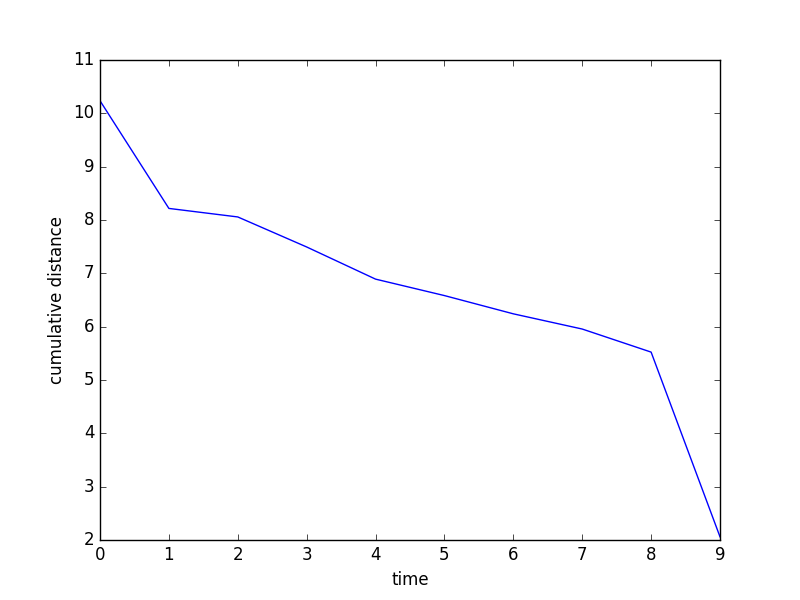
\includegraphics[width=\linewidth]{a__q_histogram}
  \captionsetup{labelformat=empty}
  \captionof{figure}{Мал. \arabic{figure}: адпаведная гістаграмма}
  \label{fig:conv-q-histogram}
\end{minipage}
\end{figure}

Агулам, у межах працы над курсавым праектаў я напісаў некалькі ўтылітаў для ROS, якія
ажыццяўлялі камунікацыі паміж ROS-кампанентамі, такія як перадача выяваў, часавых
характарыстык, геаметрычныя параметры камераў, стрымінг дадзеных у анлайн-рэжыме.

\newpage
